\section {Plataformas Blockchain}

En la actualidad, existe una amplia gama de proyectos de código abierto disponibles para la creación de aplicaciones utilizando la tecnología \textit{blockchain}. Aunque la mayor parte de éstos se encuentran relacionados a proyectos de criptomonedas, cada vez más empresas y organizaciones estudian su aplicación en escenarios distintos al del ''dinero digital'', con la finalidad de obtener beneficios (estudiados en secciones anteriores) como por ejemplo, soluciones en cadena de suministros, gestión de propiedad intelectual, administración de procesos de negocio, control de acceso e incluso plataformas de votaciones.

En esta sección se exponen dos de las plataformas más populares y estables en cuanto a documentación, trayectoria, comunidad y soporte se refiere: Ethereum e IBM Hyperledger Fabric. Ambas ofrecen un marco de trabajo (framework) ideal para el desarrollo de aplicaciones basadas en \textit{blockchaion} o DLT (por sus siglas en inglés {\it Distributed Ledger Tecnology}). Asimismo, se presenta una descripción de cada una de las tecnologías y finalmente se definen y comparan sus principales características. 


\subsection{Ethereum}
Ethreum es una red de \textit{blockchain} \textbf{pública} que posee además una criptomoneda denominada \textit{Ether}; también puede ser definida como una plataforma de código abierto que permite a los desarrolladores construir e implementar aplicaciones descentralizadas. Ethereum fue propuesto por Vitalik Buterin a finales de 2013~\cite{wood2014ethereum}, sin embargo fue lanzado oficialmente en julio de 2015. Ha ganado popularidad como plataforma de elección para muchas aplicaciones (DAPP's), así como para la creación y lanzamiento de ICO's (por sus siglas en inglés {\it Initial Coin Offering}). 

Ethereum, cuenta también con la posibilidad de creación de contratos inteligentes que definen reglas y sanciones en torno a un acuerdo, haciendo cumplir obligaciones establecidas en el mismo. En Ethereum, dichos contratos se tratan como {\it scripts} autónomos o aplicaciones descentralizadas (DAPP's) que poseen un estado que se almacena en el \textit{blockchain} para su posterior ejecución. Para su desarrollo, es posible elegir entre varios lenguajes, siendo Solidity el más recomendado. El mecanismo de consenso de Ethereum está basado en la  ''prueba de trabajo'', sin embargo, está previsto cambiarlo por la ''prueba de apuesta'', cual se encuentra en fase de prueba.

Finalmente, Ethereum utiliza una máquina virtual (EVM, por sus siglas en inglés {\it Ethereum Virtual Machine}), es decir, una computadora global distribuida donde se ejecutan todos los contratos inteligentes. Las operaciones efectuadas dentro del EVM, son ejecutadas simultáneamente por cada nodo de la red; por esta razón existe un mecanismo para limitar los recursos utilizados en cada contrato, conocido como \textit{gas}. Cada una las operaciones realizadas tiene un costo medido en gas, y cada unidad de gas consumida por una transacción debe ser pagada en \textit{Ether}.

\subsection{Hyperledger Fabric} 
Hyperledger Fabric es un proyecto avalado e impulsado por \textit{The Linux Foundation} y es mantenido actualmente por IBM~\cite{androulaki2018hyperledger}. Consiste en una infraestructura \textit{blockchain} autorizada de código abierto que proporciona una arquitectura modular y a su vez cuenta con una distinción de roles entre nodos, la cual permite la  ejecución de contratos inteligentes y servicios configurables de consenso y membresía. 

Los contratos inteligentes utilizados en Fabric son llamados ''chaincode'' y pueden estar escritos en Golang, Javascript o Java, y por lo tanto es potencialmente más flexible que un lenguaje cerrado de contratos inteligentes.

Una red Fabric está compuesta por ''pares de nodos'', los cuales son responsables de ejecutar los chaincode, acceder a los datos del \textit{blockchain}, respaldar transacciones e interactuar con aplicaciones. Dichos nodos trabajan de manera autónoma y descentralizada.

Dentro de Hyperledger Fabric, se destaca una herramienta fundamental en la agilización del desarrollo, el \textit{Hyperledger Composer}. Esta herramienta proporciona una interfaz de usuario para la configuración, implementación y prueba de una red de negocios \textit{blockchain}.

\subsection{Diferenciación y Características}

La diferencia fundamental entre Ethereum e Hyperledger se basa en su diseño y público objetivo. Ethereum con su EVM, contratos inteligentes y {\it blockchain} público, está principalmente dirigido a aplicaciones que son de naturaleza distribuida. Por otro lado Hyperledger tiene una arquitectura altamente modular y proporciona mucha flexibilidad en términos de lo que se quiere o no utilizar. Posee varios componentes y herramientas que funcionan de manera \textit{plug-and-play} y está dirigido a organizaciones o empresas que deseen optimizar sus procesos haciendo uso de la tecnología \textit{blockchain}. Por ejemplo, en Ethereum no es posible tener transacciones visibles únicamente para un usuario específico (un requisito frecuente en negocios y organizaciones) a diferencia de Fabric, el cual ofrece ésta y muchas otras herramientas al estar orientado a redes \textit{blockchain} privadas, más específicamente a ''libros contables autorizados''~\cite{blockchaintrainingalliance}.

A continuación se comparan ambas tecnologías en base a 3 aspectos fundamentales: participación de nodos, mecanismos de consenso y arquitectura general.

\subsubsection{Participación de nodos}
Implica que los nodos involucrados en la gestión del \textit{blockchain} pueden contribuir al mismo. En otras palabras, como cada nodo tiene una copia del libro distribuido en una cadena de bloques, importa cómo estos deciden sobre una verdad o estado común, volviendo obligatoria la participación de los nodos en la red.

\noindent
\textbf{Ethereum} \newline
Participación No-Autorizada: se permite la participación de cualquier persona o actor en la red, lo cual tiene sentido al ser un \textit{blockchain} público.

\textbf{Hyperledger Fabric} \newline
Participación Autorizada: los participantes se seleccionan de antemano y sólo éstos tienen acceso a la red, siendo coherente con su naturaleza privada.

\subsubsection{Mecanismos de consenso}

\noindent
\textbf{Ethereum} \newline
En Ethereum, los pares de nodos que participan en la red deben llegar a un consenso para que la transacción pueda ser agregada a la cadena de bloques. Cada nodo debe participar en el logro del consenso, incluso si no ha intervenido en la transacción efectuada. Si un nodo prueba la corrección de una transacción en la red de Ethereum, es recompensado con Ethers. Actualmente, el mecanismo de consenso se establece mediante la minería, la cual está basada en el algoritmo de ''prueba de trabajo''. Sin embargo, tras una actualización reciente conocida como Casper~\cite{buterin2017casper}, se encuentra en fase de prueba el algoritmo de consenso de tipo ''prueba de apuesta'' el  cual se espera sustituya al algoritmo de minería.

\noindent
\textbf{Hyperledger Fabric} \newline 
La definición de consenso en Fabric es diferente. No se limita a la minería basada en ''prueba de trabajo'' o cualquier otro derivado. Dado que éste opera en modo autorizado, hay un control de acceso detallado a fin de mejorar la privacidad.

Aquí, el consenso abarca todo el flujo de transacción desde el principio (propuesta de transacción) hasta el final (inclusión de la transacción dentro del \textit{blockchain}). En este caso, cada nodo asume una función diferente para lograr el consenso, a diferencia de Ethereum, donde todos los nodos tienen el mismo rol.

Los nodos se diferencian según su comportamiento:
\begin{itemize}
    \item Clientes: actúan en nombre de un usuario final; crean y por lo tanto invocan transacciones. Se comunican con  nodos ''pares'' y ''orientadores''.
    \item Pares: Mantienen el \textit{blockchain} y reciben mensajes de actualización ordenados para incluir nuevas transacciones en la plataforma. Los ''endosantes'' son un tipo especial de ''nodos pares'', cuya tarea es respaldar una transacción al verificar si cumplen con las condiciones necesarias y suficientes. (por ejemplo, suministro de firmas requeridas)
    \item Orientadores: proporcionan un canal de comunicación para los nodos clientes y pares, recibiendo y enviando mensajes que contienen la transacción que se puede transmitir.
\end{itemize}

Con Fabric, el algoritmo de consenso empleado es configurable, lo que significa que dependiendo de los requisitos específicos de la aplicación se pueden usar distintos algoritmos. Por ejemplo, para tratar con fallas de replicación aleatorias o maliciosas como se describió anteriormente, se podría usar una variante de los algoritmos de tolerancia a fallas bizantinos.

\subsubsection{Arquitectura general}
\textbf{Ethereum} \newline
El \textit{blockchain} de Ethereum tiene 2 partes principales:

\begin{itemize}
    \item Base de datos: conformada por transacciones que se almacenan en el \textit{blockchain}. Cuando un contrato es ejecutado, por ejemplo, se considera una transacción. Dichas transacciones a pesar de ser públicas (pueden ser vistas y verificadas por todos los participantes) no pueden ser alteradas de manera alguna. Finalmente, para asegurar  que todos los nodos de la red tengan la misma copia de datos, se utiliza el mecanismo de consenso anteriormente descrito, es decir, la ''prueba de trabajo'' para asegurar la plataforma.
    \item Código: en el mundo Ethereum, se escribe el código lógico o de aplicación (contrato inteligente) utilizando un lenguaje denominado Solidity. Posteriormente, se compila \textit{Ethereum Byte Code} y para finalmente implementar ese código de bytes en la plataforma \textit{blockchain}. 
\end{itemize}


Básicamente, el \textit{blockcahin} de Ethereum almacena los datos, el código y lo ejecuta en el EVM. La Figura~\ref{blockchain_ethereum_arquitecture} ilustra  la interacción con la red pública a través del EVM utilizando el paquete de interfaz js \textit{Web3js}

\begin{figure}[H]
    \centering
    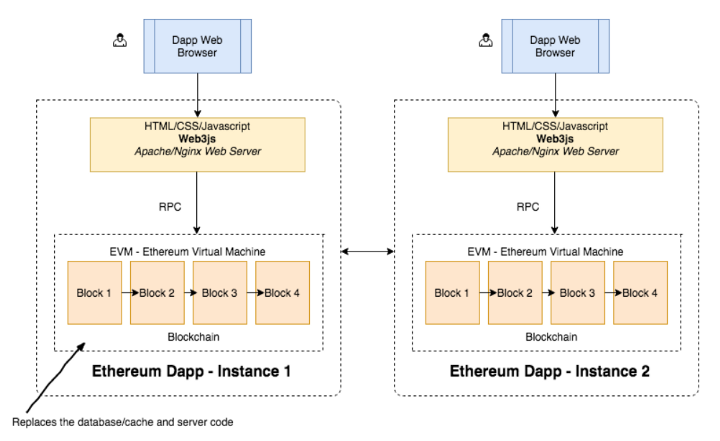
\includegraphics[width=1\textwidth]{ethereum_arquitectura.png}
     \caption{Arquitectura de Ethereum}. 
    \label{blockchain_ethereum_arquitecture}
\end{figure}

\noindent
\textbf{Hyperledger Fabric} \newline
Hyperledger Fabric presenta una arquitectura modular que permite implementaciones integrables de diversas funciones y herramientas. Uno de los elementos fundamentales del Fabric, es su ''protocolo de libro distribuido'', el cual es responsable de la integridad de datos en el \textit{blockchain} y es ejecutado por nodos. Aquí se diferencian 2 tipos de nodos:
\begin{itemize}
    \item Nodo Verificador: es un nodo en la red responsable de ejecutar el consenso, validar las transacciones y mantener el libro contable.
    \item Nodo No-Verificador: es un nodo que funciona como un proxy para conectar clientes (emitir transacciones) con nodos verificadores.
\end{itemize}

Como se mencionó en la sección de mecanismos de consenso, los ''nodos verificadores'' realizan un protocolo a prueba de ''fallas bizantinas'' para ejecutar una máquina de estado distribuido la cual acepta tres tipos de transacciones: implementación, invocación y consulta. La primera, hace referencia a la instalación de un chaincode dentro de un nodo; la segunda ejecuta el chaincode previamente instalado en el nodo (generando posibles cambios de estado) y la última, se refiere a la consulta de estado actual sobre el \textit{blockchain}.

Al estar enfocado en la implementación de libros contables autorizados, Fabric admite la autorización de inscripción y uso de transacciones a través de certificados de clave pública, y la confidencialidad para el chaincode (contratos inteligentes) ejecutados a través de cifrado \textit{in-band}.

En la Figura~\ref{blockchain_fabric_arquitecture}, se visualiza un ejemplo de aplicación de cuidados médicos soportada en Fabric. De lado derecho se aprecia su configuración física, del lado derecho sus componentes lógicos: permisología, nodos, consenso.

\begin{figure}[H]
    \centering
    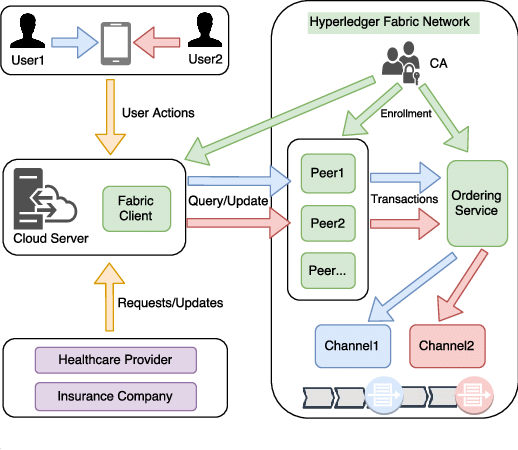
\includegraphics[width=0.8\textwidth]{fabric-arquitectura.png}
     \caption{Arquitectura de Fabric.} 
    \label{blockchain_fabric_arquitecture}
\end{figure}

Finalmente se presenta una tabla comparativa en la Figura ~\ref{blockchain_ethereum_hyperledger}  entre las dos plataformas con las características mas relevantes.

\begin{figure}[H]
    \centering
    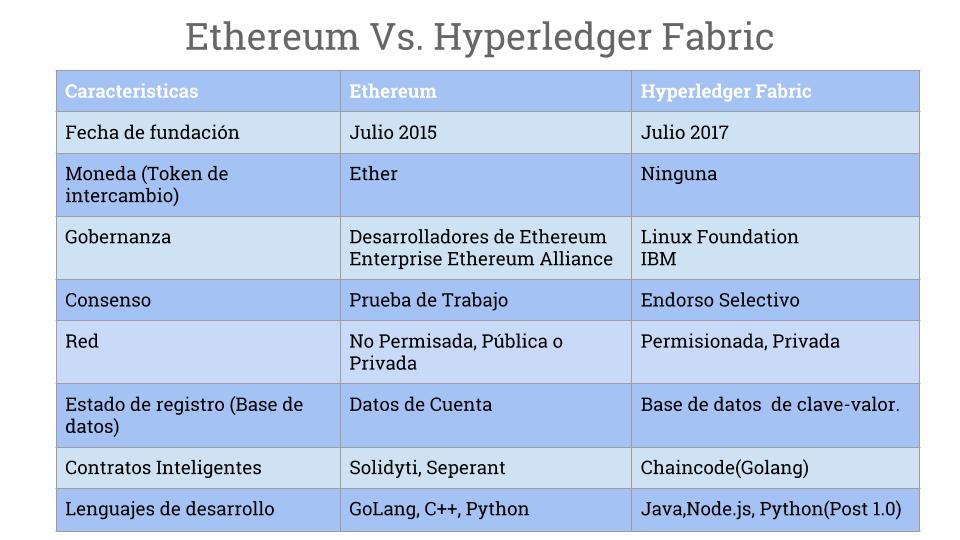
\includegraphics[width=1\textwidth]{Figs/Chapter2/ethereum_vs_hyperledger.jpg}
     \caption{Ethereum Vs. Hyperledger Fabric.} 
    \label{blockchain_ethereum_hyperledger}
\end{figure}
